\documentclass[10pt, compress]{beamer}

\usetheme{m}

\usepackage{booktabs}
\usepackage[scale=2]{ccicons}
\usepackage{minted}
\usepackage{graphicx}

\usepgfplotslibrary{dateplot}

\usemintedstyle{trac}

\title{ParKazoo}
\subtitle{Implementing a partitioned ZooKeeper using Kazoo}
\date{\today}
\author{Arjun Naik}
\institute{TU Dresden}

\begin{document}

\maketitle

\section{Introduction}

\begin{frame}[fragile]
    \frametitle{ZooKeeper}
    A service for coordinating processes of distributed applications.
    \begin{quote}
        ZooKeeper aims to provide a simple and high performance kernel for building more complex
        coordination primitives at the client. 
    \end{quote}
\end{frame}

\begin{frame}[fragile]
    \frametitle{ZooKeeper Architecture}
    \begin{figure}[ht!]
        \centering
        \includegraphics[width=100mm]{images/ZKArchWithoutBG.png}
        \caption{A simple caption \label{overflow}}
    \end{figure}
\end{frame}

\begin{frame}[fragile]
    \frametitle{ParKazoo}
    \begin{itemize}
        \item Pure Python Implementation
        \item Supports Gevent (single threaded IO Loop)
        \item Implements many of the popular recipes.
    \end{itemize}
\end{frame}

\begin{frame}[fragile]
    \frametitle{Primary Order}
    \begin{itemize}
        \item All operations from client are executed in order.
        \item Full primary order cannot be preserved.
        \item Primary order on sibling preserved.
    \end{itemize}
\end{frame}

\section{Approach}
\begin{frame}[fragile]
    \frametitle{Partitioned Architecture}
    \begin{figure}[ht!]
        \centering
        \includegraphics[width=70mm]{images/ParKazooArchWithoutBG.png}
        \caption{ParKazoo Ensemble \label{overflow}}
    \end{figure}
\end{frame}

\begin{frame}[fragile]
    \frametitle{Partitioned Architecture}
    \begin{itemize}
        \item Multiple Clusters
        \item Single Ensemble
        \item Every client connects to every Cluster
        \item Connections are distributed over Clusters
        \item Linear speedup can be achieved.
    \end{itemize}
\end{frame}

\begin{frame}[fragile]
    \frametitle{Assigning Node to cluster}
    Path of parent is used to calculate the destionation cluster.
    \begin{equation}
        Destination Cluster = hash(Parent Path) \% len(Num. of Clusters)
    \end{equation}
    Sibling nodes get mapped to the same cluster.
\end{frame}

\begin{frame}[fragile]
    \frametitle{Creating a Node}
    \begin{itemize}
        \item Check if the parent exists on its cluster.
        \item Check if parent is ephemeral
        \item If everything ok, then create the Node.
    \end{itemize}
    \begin{figure}[ht!]
        \centering
        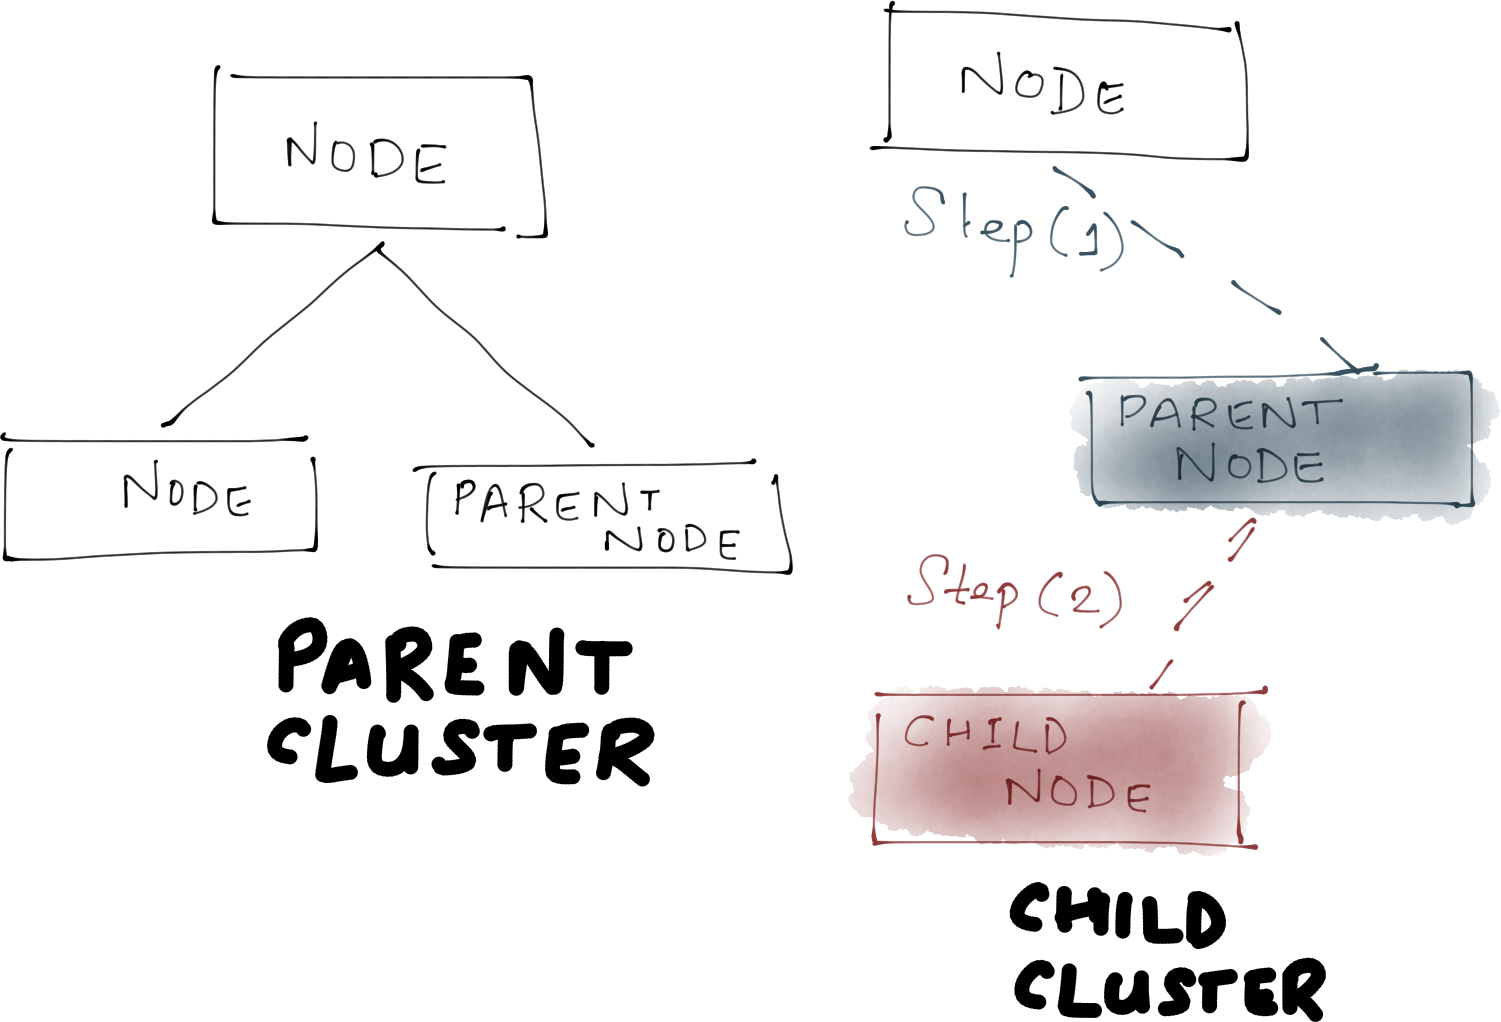
\includegraphics[width=60mm]{images/ParKazooCreate.png}
    \end{figure}
\end{frame}

\begin{frame}[fragile]
    \frametitle{Getting Children of Node}
    \begin{itemize}
        \item All children of Node on single cluster.
        \item Check if node exists
        \item Check if the path exists on children cluster.
        \item If not create it, so that watches can be left.
    \end{itemize}
\end{frame}

\begin{frame}[fragile]
    \frametitle{Deleting a Node}
    \begin{itemize}
        \item Delete can be recursive.
        \item Then delete from all clusters.
        \item If not recursive, then check if node has children.
    \end{itemize}
\end{frame}

\section{Proof}
\begin{frame}
\end{frame}

\section{Measurements}
\begin{frame}
\end{frame}

\plain{Questions?}

\end{document}
